\documentclass[12pt]{article}
\usepackage[margin=1in]{geometry}
\usepackage[T1]{fontenc}
\usepackage[utf8]{inputenc}
\usepackage{textcomp}
\usepackage{newtxtext,newtxmath}
\usepackage{graphicx}
\usepackage{booktabs}
\usepackage{array}
\usepackage{longtable}
\usepackage{float}
\usepackage{caption}
\usepackage{setspace}
\usepackage{xcolor}
\usepackage{hyperref}
\usepackage{bookmark}
\doublespacing
\setlength{\parindent}{0pt}
\setlength{\parskip}{0pt}
\setlength{\emergencystretch}{3em}
\newcommand{\tablecaptionfontsize}{\fontsize{10pt}{12pt}\selectfont}
\newcommand{\tablefontsize}{\fontsize{9pt}{11pt}\selectfont}
\DeclareCaptionFont{captionten}{\fontsize{10pt}{12pt}\selectfont}
\captionsetup{
  font=captionten,
  labelfont=bf,
  textfont=captionten,
  justification=raggedright,
  labelsep=period,
  singlelinecheck=false
}
\newcolumntype{L}[1]{>{\tablefontsize\raggedright\arraybackslash}m{#1}}
\renewcommand{\thefigure}{S\arabic{figure}}
\renewcommand{\thetable}{S\arabic{table}}
\urlstyle{same}
\hypersetup{
  pdftitle={Supplementary Material},
  hidelinks,
  pdfcreator={LaTeX}
}

\begin{document}

\begin{center}
{\LARGE Supplementary Material}
\end{center}

This supplementary material lists implementation details used in the GrapeMaster platform. The main manuscript reports the platform architecture, data flow, analytical modules, validation design, and workflow verification; this document provides supplementary linkage figures, database relationship rules, workflow verification rules, the software stack, selected data-model attributes, and operational-record screening rules for reproducibility and technical inspection.

\section*{Supplementary figures}

\begin{figure}[H]
\centering
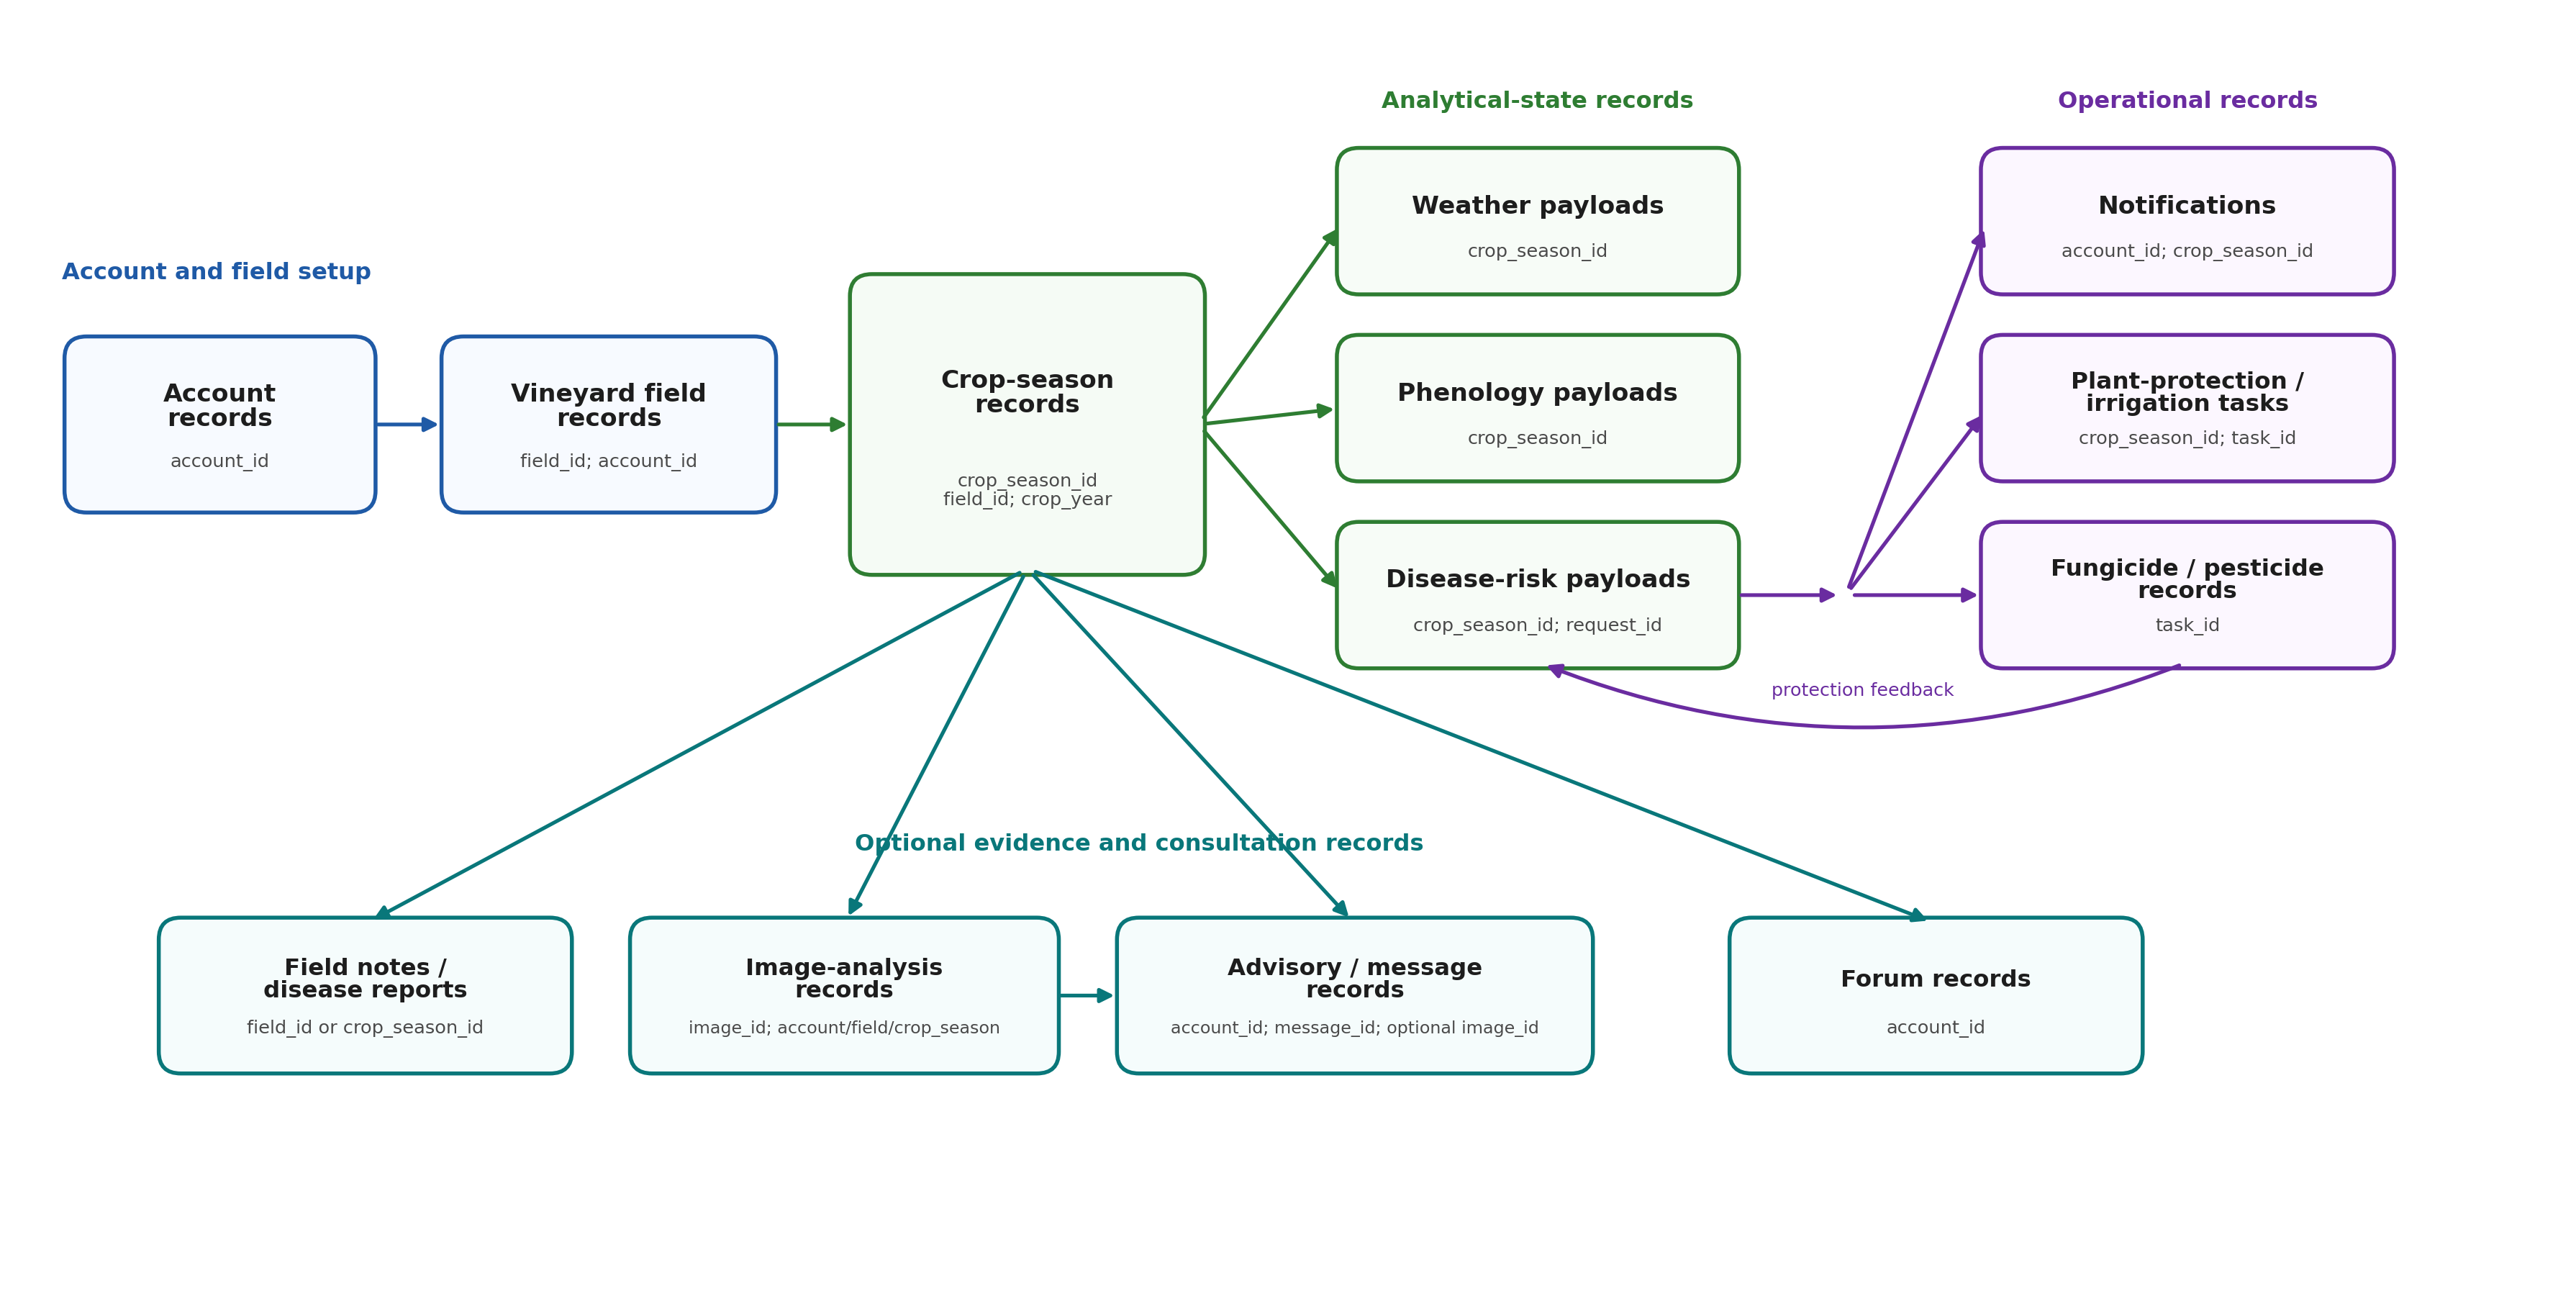
\includegraphics[width=\linewidth]{../fig/grapemaster_backend_identifier_linkage.png}
\caption{Backend identifier linkage among GrapeMaster record classes. The crop-management record is shown as a data-linkage object connecting field setup with time-dependent analytical and operational records. Task identifiers directly connect field operations with product-level treatment feedback; image and advisory records use the available account, field, crop, image, or message context. The figure is a schematic linkage view and does not report deployment counts or causal relationships.}
\label{fig:supp_backend_operational_linkage}
\end{figure}

\begin{figure}[H]
\centering
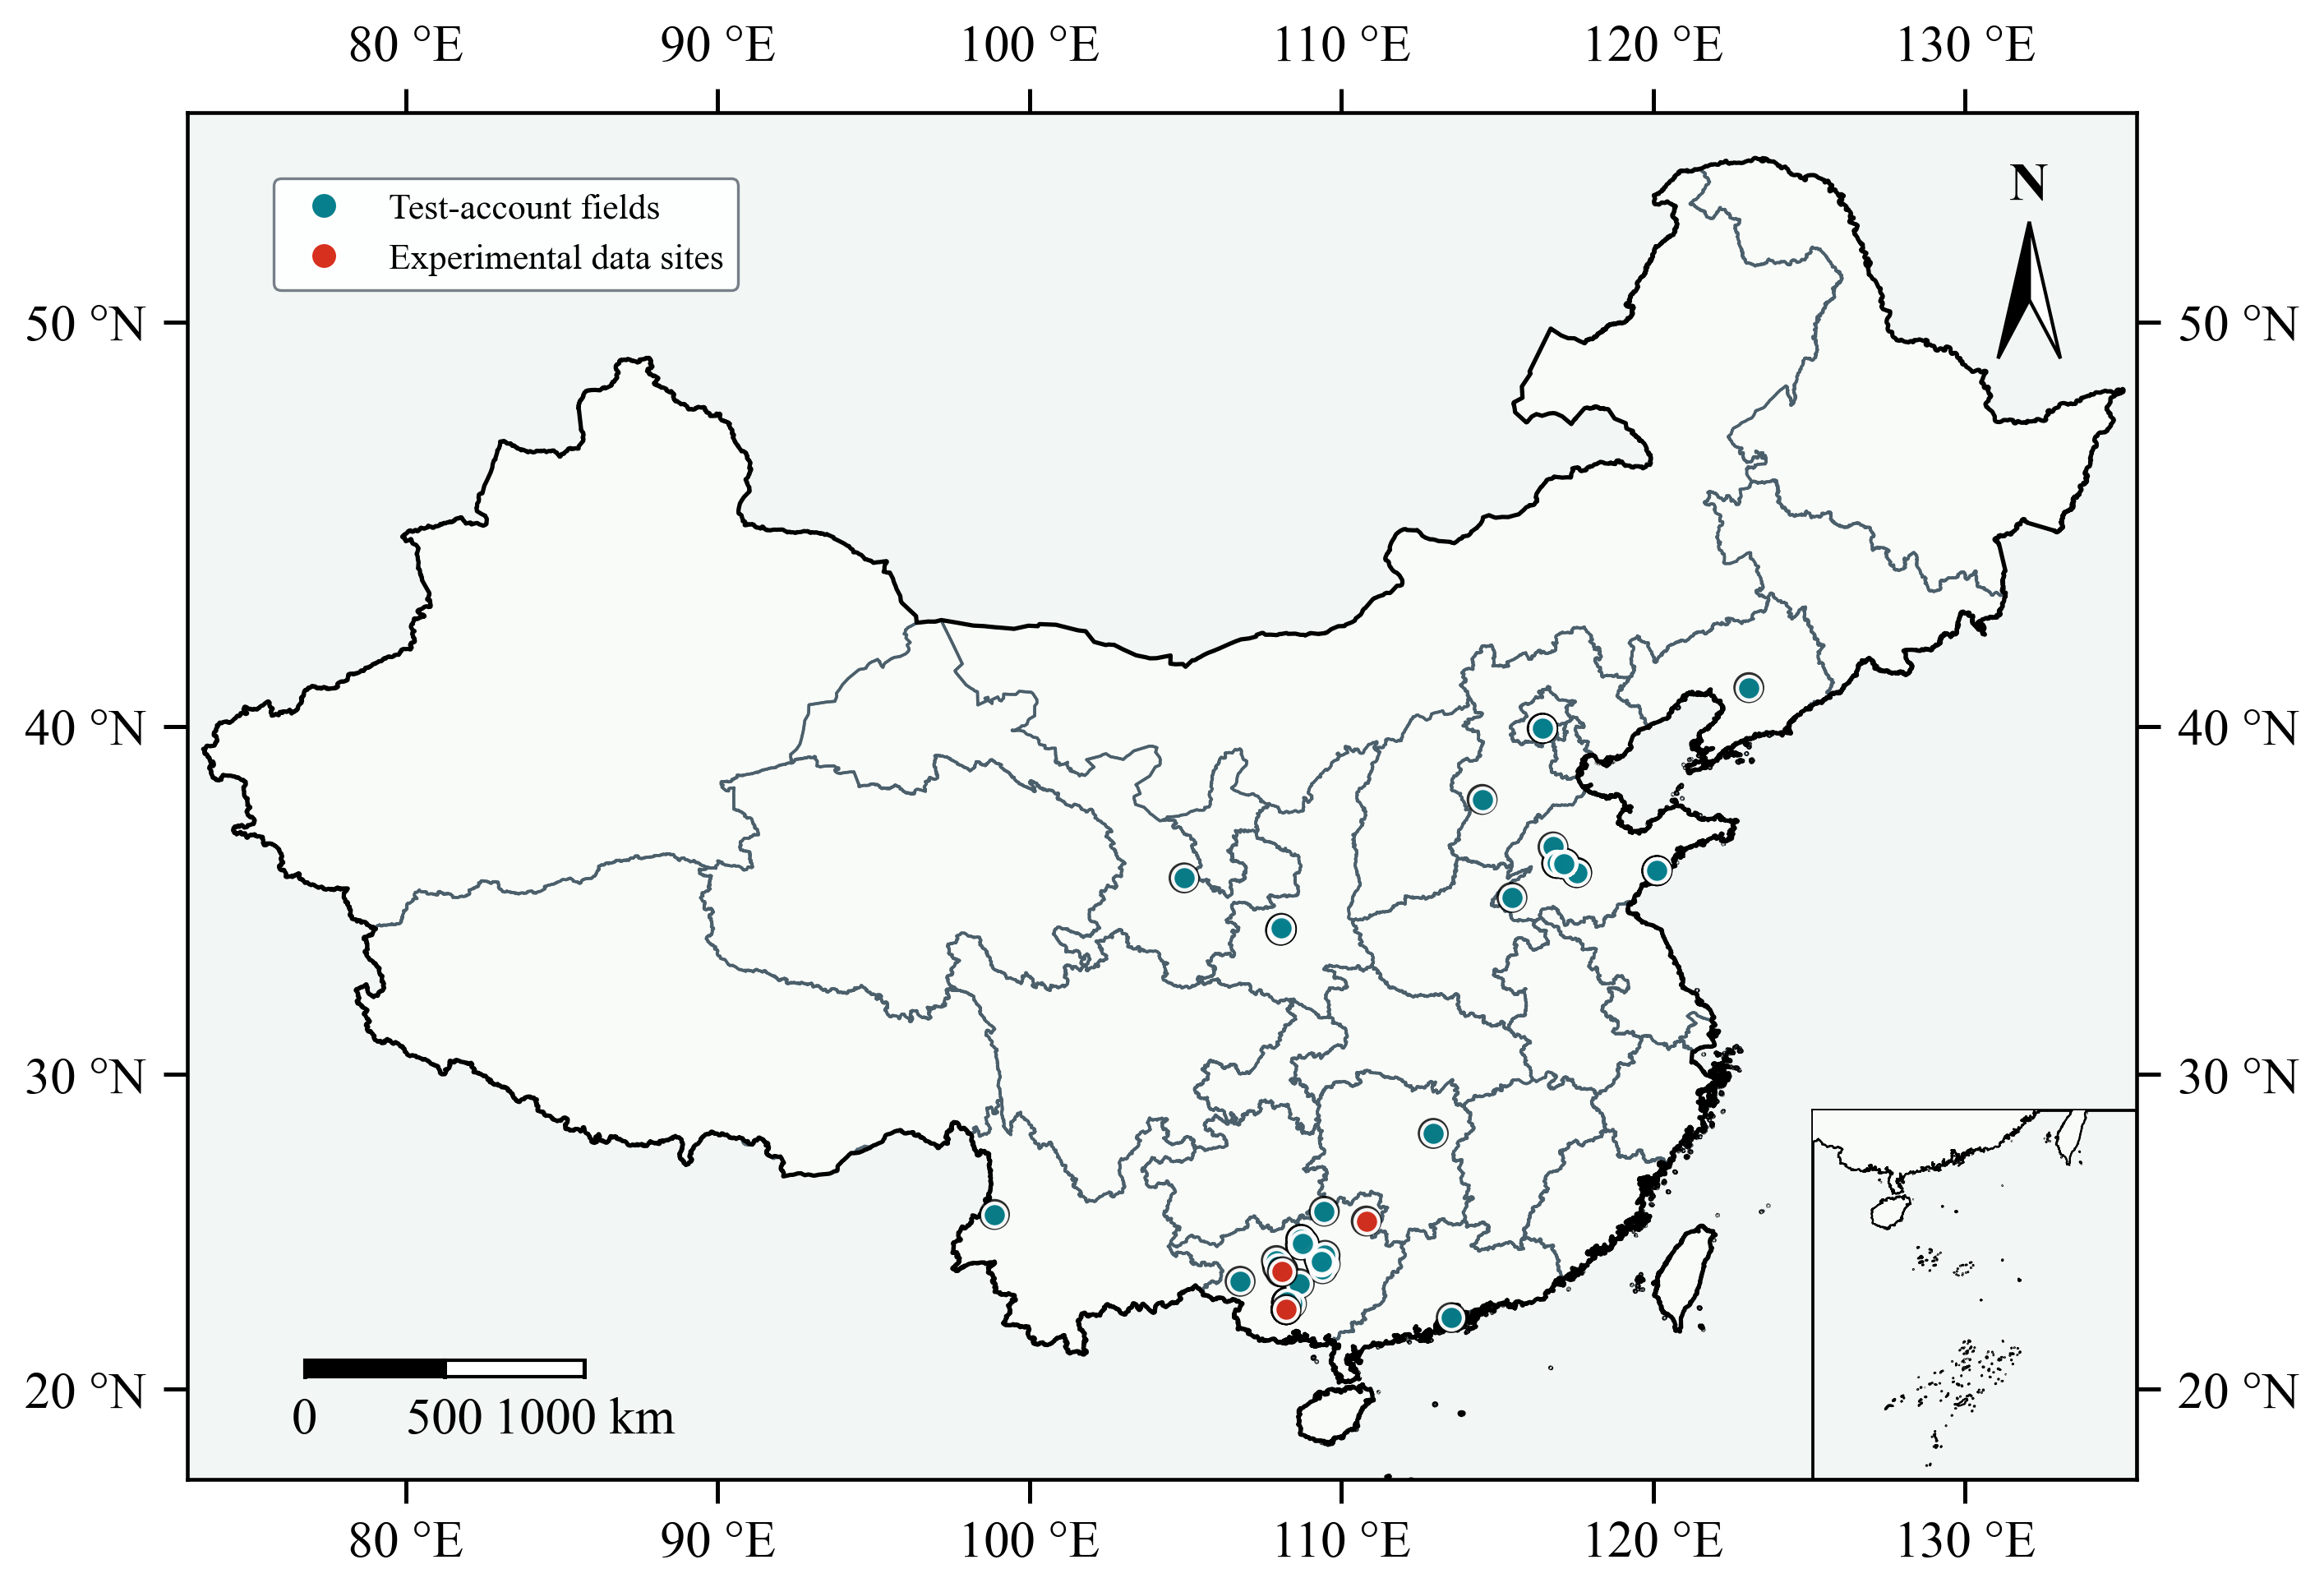
\includegraphics[width=\linewidth]{../fig/grapemaster_test_site_distribution_map.png}
\caption{Spatial context of mappable platform field records and independent experimental module-validation sites. Teal bubbles show mappable field records aggregated by region, with bubble size indicating the number of records per region. Red points indicate experimental sites used for module-level validation and are not part of the operational-record denominator.}
\label{fig:supp_platform_field_distribution}
\end{figure}

\section*{Supplementary tables}

\begingroup
\setlength{\tabcolsep}{3pt}
\renewcommand{\arraystretch}{1.12}
\begin{longtable}{@{}L{0.22\linewidth} L{0.37\linewidth} L{0.33\linewidth}@{}}
\caption{Input-output definitions and calibration notes for platform-compatible analytical components.}\label{tab:supp_module_details}\\
\toprule
Module & Inputs and outputs & Workflow position and calibration note \\
\midrule
\endfirsthead
\toprule
Module & Inputs and outputs & Workflow position and calibration note \\
\midrule
\endhead
Phenology service & Inputs include crop-season metadata, cultivar and cultivation context, and date-aligned daily temperature or weather series. Outputs include broad BBCH-related growth-stage states, stage timelines, and daily crop-stage sequences. & Provides host-development context for susceptibility interpretation, warning-window definition, task timing, and mobile display. The implementation is a Guangxi-calibrated adaptation of temperature-driven grapevine phenology modelling; parameter thresholds and validation metrics are retained as module-level configuration. \\
FSIM-S risk service & Inputs include transformed hourly or daily weather, crop-stage sequence, cultivar susceptibility, target-disease settings, and recent fungicide-history records. Outputs include downy mildew disease-risk states, first-infection warning triggers, treatment-window information, and protection-state interpretation. & Supplies pre-symptomatic risk information to the proactive management workflow. The evaluated configuration is locally calibrated for humid subtropical Guangxi vineyards. Field-derived sporangia pressure is used as an optional model-level calibration or sensor-enhanced pathway, not as a required live input for routine operation. \\
Image-recognition service & Inputs include user-uploaded grape symptom images. Outputs include disease or healthy categories, confidence values, and stored image-analysis records. & Supplies post-symptomatic diagnostic evidence to the mobile application. Candidate visual models were evaluated with grape-focused validation metrics, including accuracy, precision, recall, and F1-score. \\
LLM-assisted advisory service & Inputs include advisory text and available diagnostic or management context. Outputs include management-oriented advisory text and stored advisory records. & Supplies contextual explanation and conversational advisory support after image recognition or user questioning. The service follows the CDIP-ChatGLM3 framework and is not used as a substitute for validated disease models, expert diagnosis, pesticide labels, or local regulations. \\
\bottomrule
\end{longtable}
\endgroup

\begingroup
\setlength{\tabcolsep}{3pt}
\renewcommand{\arraystretch}{1.12}
\begin{longtable}{@{}L{0.23\linewidth} L{0.36\linewidth} L{0.33\linewidth}@{}}
\caption{Database relationship rules supporting model-to-management workflow reconstruction.}\label{tab:supp_database_relationship_rules}\\
\toprule
Relationship rule & Required linkage & Verification purpose \\
\midrule
\endfirsthead
\toprule
Relationship rule & Required linkage & Verification purpose \\
\midrule
\endhead
Account-to-field linkage & Retained account identifiers must link to at least one vineyard field record & Confirms that the account has an operational vineyard context rather than registration-only activity \\
Field-to-crop linkage & Each evaluated crop-management record must be linked to a field record through field or crop identifiers & Separates persistent field identity from time-dependent analytical and management state \\
Crop-to-analytical-payload linkage & Weather, phenology, disease-risk, and model request-response payloads should share the crop identifier where applicable & Confirms that model inputs and outputs can be retrieved under the same management context \\
Context-to-event linkage & Notifications, warning events, and task records should be associated with the retained user, field, or crop context & Confirms contextual association without implying direct event-to-task causality \\
Task-to-product linkage & Fungicide or pesticide product records must link to plant-protection tasks through task identifiers & Confirms that completed operations can be converted into product-level treatment feedback \\
Symptom/advisory context linkage & Image records, advisory records, field notes, and disease reports should retain available account, field, crop, image, or message identifiers & Confirms whether symptom-related records and advisory interactions can be retrieved with relevant management information \\
Explicit absence rule & If an expected optional record type is absent for a replay anchor, the absence is recorded rather than inferred as failure of unrelated workflow steps & Prevents overclaiming and separates missing symptom or advisory records from successful risk-task-feedback linkage \\
\bottomrule
\end{longtable}
\endgroup

\begingroup
\setlength{\tabcolsep}{3pt}
\renewcommand{\arraystretch}{1.12}
\begin{longtable}{@{}L{0.24\linewidth} L{0.36\linewidth} L{0.32\linewidth}@{}}
\caption{Workflow verification rules used for operational-record and representative-replay checks.}\label{tab:supp_verification_rules}\\
\toprule
Verification check & Operational criterion & Supported interpretation \\
\midrule
\endfirsthead
\toprule
Verification check & Operational criterion & Supported interpretation \\
\midrule
\endhead
Operational-account retention & An account is retained only when it has business records and field-crop-season linkage after deduplication and target-context screening & Defines the evaluated operational account set \\
Analytical payload completeness & A crop season is counted as analytically complete when weather, phenology, disease-risk, and request-response payloads are present under the shared seasonal context & Shows whether the analytical state can be reconstructed for that season \\
Disease-risk-to-operation linkage & Notification and task records are checked against retained user, field, or crop-season context & Shows whether disease-risk or management events entered the operational workflow \\
Treatment-feedback linkage & Fungicide or pesticide records are checked through task identifiers and task completion status & Shows whether field operations can be converted into feedback records \\
Symptom/advisory record-linkage availability & Image-analysis, advisory, disease-report, and note records are checked for available account, field, crop-season, image, or message links & Shows whether symptom-related records and advisory interactions are available for seasonal interpretation \\
Representative replay & A selected crop-season anchor must retrieve weather, phenology, disease-risk, notification, task, and fungicide records through shared crop-season or task keys & Demonstrates reconstructability of one disease-risk-to-feedback chain \\
Boundary reporting & Missing optional symptom or advisory records under the replay anchor are explicitly reported rather than omitted & Separates verified linkage from unsupported production-outcome claims \\
Excluded outcome claim & Operational-record linkage and replay checks are not treated as demonstrations of pesticide reduction, disease-control efficacy, economic benefit, or user adoption & Maintains the distinction between record-based workflow assessment and agronomic-impact evaluation \\
\bottomrule
\end{longtable}
\endgroup

\begingroup
\setlength{\tabcolsep}{3pt}
\renewcommand{\arraystretch}{1.12}
\begin{longtable}{@{}L{0.20\linewidth} L{0.29\linewidth} L{0.19\linewidth} L{0.22\linewidth}@{}}
\caption{Record-level reconstruction results for a loop-complete crop-season replay in GrapeMaster.}\label{tab:supp_crop_season_replay_audit}\\
\toprule
Record group & Retained record set & Identifier or status & Result note \\
\midrule
\endfirsthead
\toprule
Record group & Retained record set & Identifier or status & Result note \\
\midrule
\endhead
Replay record set & Weather, phenology, disease-risk, notification, task, and fungicide records & One crop-season UUID & Loop-complete crop-season replay \\
State and risk records & Weather, phenology, and disease-risk payloads & Shared crop-season key & Shared seasonal record set \\
Operation records & Notifications and completed plant-protection tasks & Same crop-season context & Notification and task records \\
Treatment-feedback records & Fungicide-product records & Task identifiers & Product-task record set \\
Field-note branch & No field-note or incidence-note record & Explicit absence & No field/incidence note in this replay \\
\bottomrule
\end{longtable}
\endgroup

\begingroup
\setlength{\tabcolsep}{3pt}
\renewcommand{\arraystretch}{1.12}
\begin{longtable}{@{}L{0.20\linewidth} L{0.30\linewidth} L{0.42\linewidth}@{}}
\caption{Software stack and implementation components used in the GrapeMaster platform.}\label{tab:supp_software_stack}\\
\toprule
Layer & Component group & Main technologies or libraries \\
\midrule
\endfirsthead
\toprule
Layer & Component group & Main technologies or libraries \\
\midrule
\endhead
Mobile client & Application framework & Dart, Flutter \\
Mobile client & Android shell and build configuration & Kotlin, Gradle \\
Backend business service & Web framework and API layer & Python, Django 4.2, Django REST Framework \\
Backend business service & Authentication, scheduling, and asynchronous communication & SimpleJWT, Django APScheduler, Django Channels \\
Backend business service & Database access and persistence & PostgreSQL, \texttt{psycopg2}, normalized relational tables, JSON model payloads \\
Disease-model service & Service interface & FastAPI, Uvicorn, Pydantic, Starlette \\
Weather and time-series processing & Numerical and date-time processing & NumPy, Pandas, Python Dateutil, Pytz \\
Weather and geospatial processing & Field geometry, geocoding, and configured weather-service access & Shapely, Fiona, GeoPandas, Geopy, Requests, HTTPX, weather-service client packages, request caching, retry utilities \\
Phenology and risk analytics & Crop-stage and risk-state calculation & Python analytical workflows, date-aligned weather transformation, cultivar and crop-season metadata \\
Image processing and recognition & Image preprocessing and deep-learning inference & PyTorch, TorchVision, OpenCV, Pillow, Ultralytics-related components, EfficientViT-related modules, segmentation components \\
Advisory interface & Text advisory channel & ChatGLM3-derived advisory workflow following the published CDIP-ChatGLM3 framework \\
\bottomrule
\end{longtable}
\endgroup

\begingroup
\setlength{\tabcolsep}{3pt}
\renewcommand{\arraystretch}{1.12}
\begin{longtable}{@{}L{0.23\linewidth} L{0.31\linewidth} L{0.38\linewidth}@{}}
\caption{Selected data-model attributes supporting model-to-management integration.}\label{tab:supp_data_model_attributes}\\
\toprule
Record group & Main attributes or stored content & Platform role \\
\midrule
\endfirsthead
\toprule
Record group & Main attributes or stored content & Platform role \\
\midrule
\endhead
Field record & User linkage, field name, area, GeoJSON boundary, centroid coordinates, administrative region, sharing state, deletion state, notice state, and generated field-boundary preview & Persistent spatial and ownership unit for vineyard management \\
Field geometry processing & Boundary parsing, boundary-image generation, area estimation, centroid calculation, and optional geocoding request & Converts user-defined field boundaries into location and display objects \\
Crop-management record & Field linkage, grape cultivar, cultivation method, vine age, field coordinates, field size, and cultivar metadata & Time-dependent execution and retrieval key for analytical and operational records \\
Master-data records & Grape variety, cultivar susceptibility, cultivation method, BBCH stage, disease type, fungicide, pesticide, and reminder rules & Controlled reference values for field, crop, task, risk, and advisory records \\
Model payload records & Weather, phenology, disease-risk, and request-response payloads stored with structured records & Preserves inputs and outputs for mobile display, recalculation, and audit \\
\bottomrule
\end{longtable}
\endgroup

\begingroup
\setlength{\tabcolsep}{3pt}
\renewcommand{\arraystretch}{1.12}
\begin{longtable}{@{}L{0.25\linewidth} L{0.43\linewidth} L{0.24\linewidth}@{}}
\caption{Operational-record screening rules used before summarizing deployed GrapeMaster records.}\label{tab:supp_screening_rules}\\
\toprule
Screening step & Rule & Rationale \\
\midrule
\endfirsthead
\toprule
Screening step & Rule & Rationale \\
\midrule
\endhead
User-record integration & User records were integrated using available user identifier, custom-user identifier, and phone-number fields. & Avoids duplicate counting of account-level records \\
Business-record filter & Accounts with no business records across field, crop-season, notification, task, fungicide or pesticide, advisory or message, forum, disease-report, and note tables were excluded. & Removes registration-only accounts from operational summaries \\
Field-crop linkage filter & Accounts without both field records and crop-management records were excluded. & Retains records that can support implemented workflow reconstruction \\
Target-context filter & A single account associated only with Linwei District was excluded. & Removes a non-target-region account from the Guangxi vineyard evaluation context \\
Retained account set & Forty-seven accounts remained from 95 deduplicated accounts. & Defines the candidate account set used for operational-record coverage \\
\bottomrule
\end{longtable}
\endgroup
\end{document}
